\section{Tachysséma Développement}
\subsection{Présentation de la Société}

Dans le cadre du master SME, je réalise ma première année d'alternance au sein de la SARL TACHYSSEMA DEVELOPPEMENT basée à Labège (31).
Cette société est spécialisée dans le traitement vidéo et le traitment du signal en temps réel pour des systèmes éléctroniques embarqués. 

En conséquence, la société possède un rayon d'action étendu qui comprend de la R\&D, du développement matériel (caméras embarqués, conception de cartes éléctroniques) et du dévellopement logiciel. 

Les domaines d'applications de la société est également varié puisque la société peut être amenée à réaliser des projet en lien avec l'aéronotique, le secteur médical, militaire ou encore automobile. 



\subsection{Organisation interne}

Les locaux de Tachysséma Développement sont partagés avec Visif Technology, une société spécialisée dans le dévellopement de solutions technologiques pour les énergies renouvelables. Cependant les deux sociétés possèdes des projets communs et travaillent ensembles. 

Au sein de Tachysséma Développement, Nicolas Roddier, mon tuteur d'alternance et gérant de la société est assité par un ingénieur en automatique ainsi qu'une stagiaire M2 SME, un alternant en M2 SME et moi même. 

Pour Visif Technology, sont présents 

Il 



\newpage

\section{Projets Réalisés}
Dans cette partie nous réaliserons la synthése des projets principaux menés depuis mon arrivé chez Tachysséma Développement, en octobre 2019. 

\subsection{Réalisation d'une IHM avec l'environnement GTK}

Dans le cadre d'un projet de gestion et contrôle de pixels deffectueux présents sur un capteur d'une caméra, j'ai réalisé une interface homme machine permettant de réaliser l'interface entre l'utilisateur et un module FPGA qui contrôle le capteur d'une caméra. 
\\ 

\subsubsection{Contexte} 

Le capteur d'une caméra est constitué d'un ensemble pixels qui captent la lumière entrante. On peut représenter l'ensemble de ces pixels sous la forme d'une matrice. Avec le temps, il est possible que certains pixels deviennent deffectueux, on parle alors de pixels morts. Les pixels deffectueux doivent pouvoir être localisés, corigés ou remplacés.  
\newline

La caméra est composée d'un FPGA qui contrôle le capteur vidéo. Il permet notament de réaliser le traitement des pixels deffectueux. L'interface homme machine interragit avec le FPGA, elle permettra la réalisations des actions de lectures et d'écriture dans une mémoire EEPROM qui contient les coordonnés matricielle des pixels morts. 

\subsubsection{Cahier des charges de l'IHM } 

\begin{figure}[ht]
	\centering
    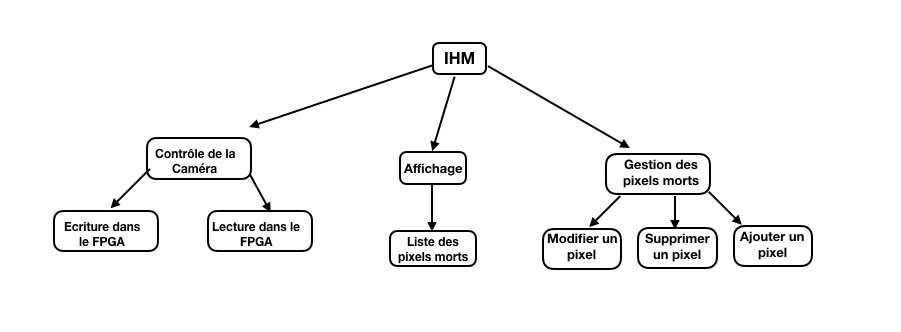
\includegraphics[scale=0.5]{img/cdcIHM.png}
    \caption{Générateur MAVGEN}
    \label{fig:mavgen}
\end{figure}

Voici ci-dessous les principales fonctions qui sont réalisées par l'IHM : 
\newline
\begin{itemize}
	\item L'utilisateur peut lire et écrire la liste des pixels déffectueux dans un fichier .txt qui est sauvegardé sur le disque dur de l'ordinateur (ou est executée l'IHM). 
	\item L'IHM peut intérragir avec la caméra par le biais d'une communication série. Elle réalise des opérations de lectures et d'écritures dans une table FPGA ainsi que dans une mémoire EEPROM qui contient les coordonnées des pixels défectueux. 
	\item Une fois que les coordonnés des pixels morts sont chargés de la caméra vers l'IHM ou du fichier .txt vers l'IHM, cette dernière les affiches sous la forme d'une liste comportant deux colonnes (une pour la ligne et une pour la colonne du pixel mort). 
	\item L'utilisateur peut effectuer différentes actions sur la liste des mauvais pixels. Il peut notament ajouter, supprimer ou remplacer des pixels deffectueux. A chaque modification, la liste est actualisée et transmise au FPGA.

\end{itemize}

\subsubsection{Implémentation}

\begin{figure}[ht]
    \centering
    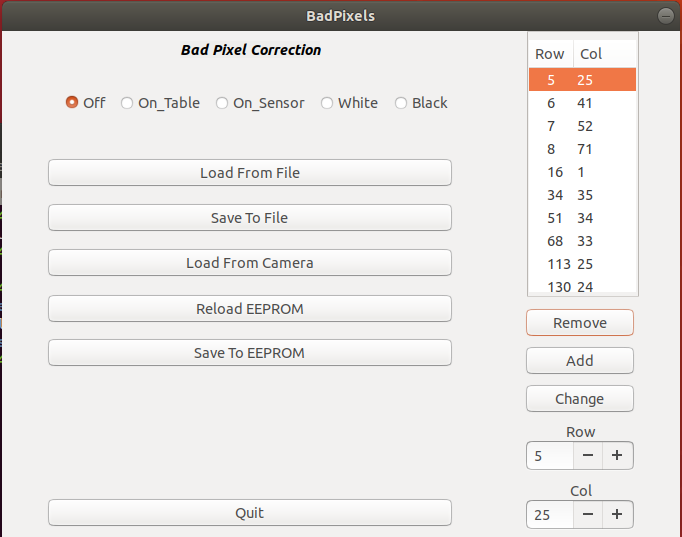
\includegraphics[scale=0.45]{img/IHM.png}
    \caption{Apperçu de l'IHM}
    \label{fig:CameraCmdsettings}
\end{figure}

\subsubsubsection{Interface graphique}

La première étape que j'ai effectué sur ce projet est la réalisation de la partie graphique de l'IHM. Cette dernière devait s'éxecuter sur une distribution linux.

En conséquence j'ai utilisé l'outil de développement graphique Glade qui intègre GTK+. Glade permet facilité la réalisation d'interface graphique: En effet on vient placer les différents objets ( boutons, champs de texte, curseurs etc .. ) sans passer par le code. 

Une fois ce processus terminé, glade génrère la solution obtenu dans un fichier .XML que nous pouvons intégrer directement dans un langage de programmation ( C, C++, Pyhton et d'autres encore). 
\newline

\subsubsubsection{Implémentation du code}

Ensuite j'ai pu implémenté le code en langage C ce qui permet d'établir un lien entre un évement lié à l'interface graphique ( appuie sur un bouton, changement de valeur sur un curseur ..) et une fonction répondant au cahier des charges ( envoie des données dans le FPGA, quitter l'IHM ou encore écrire le fichier .txt par exemple). 



\subsection{Projet WindFloat Atlantic : Traitement des données d'un équipement embarqué}

\begin{figure}[ht]
    \centering
    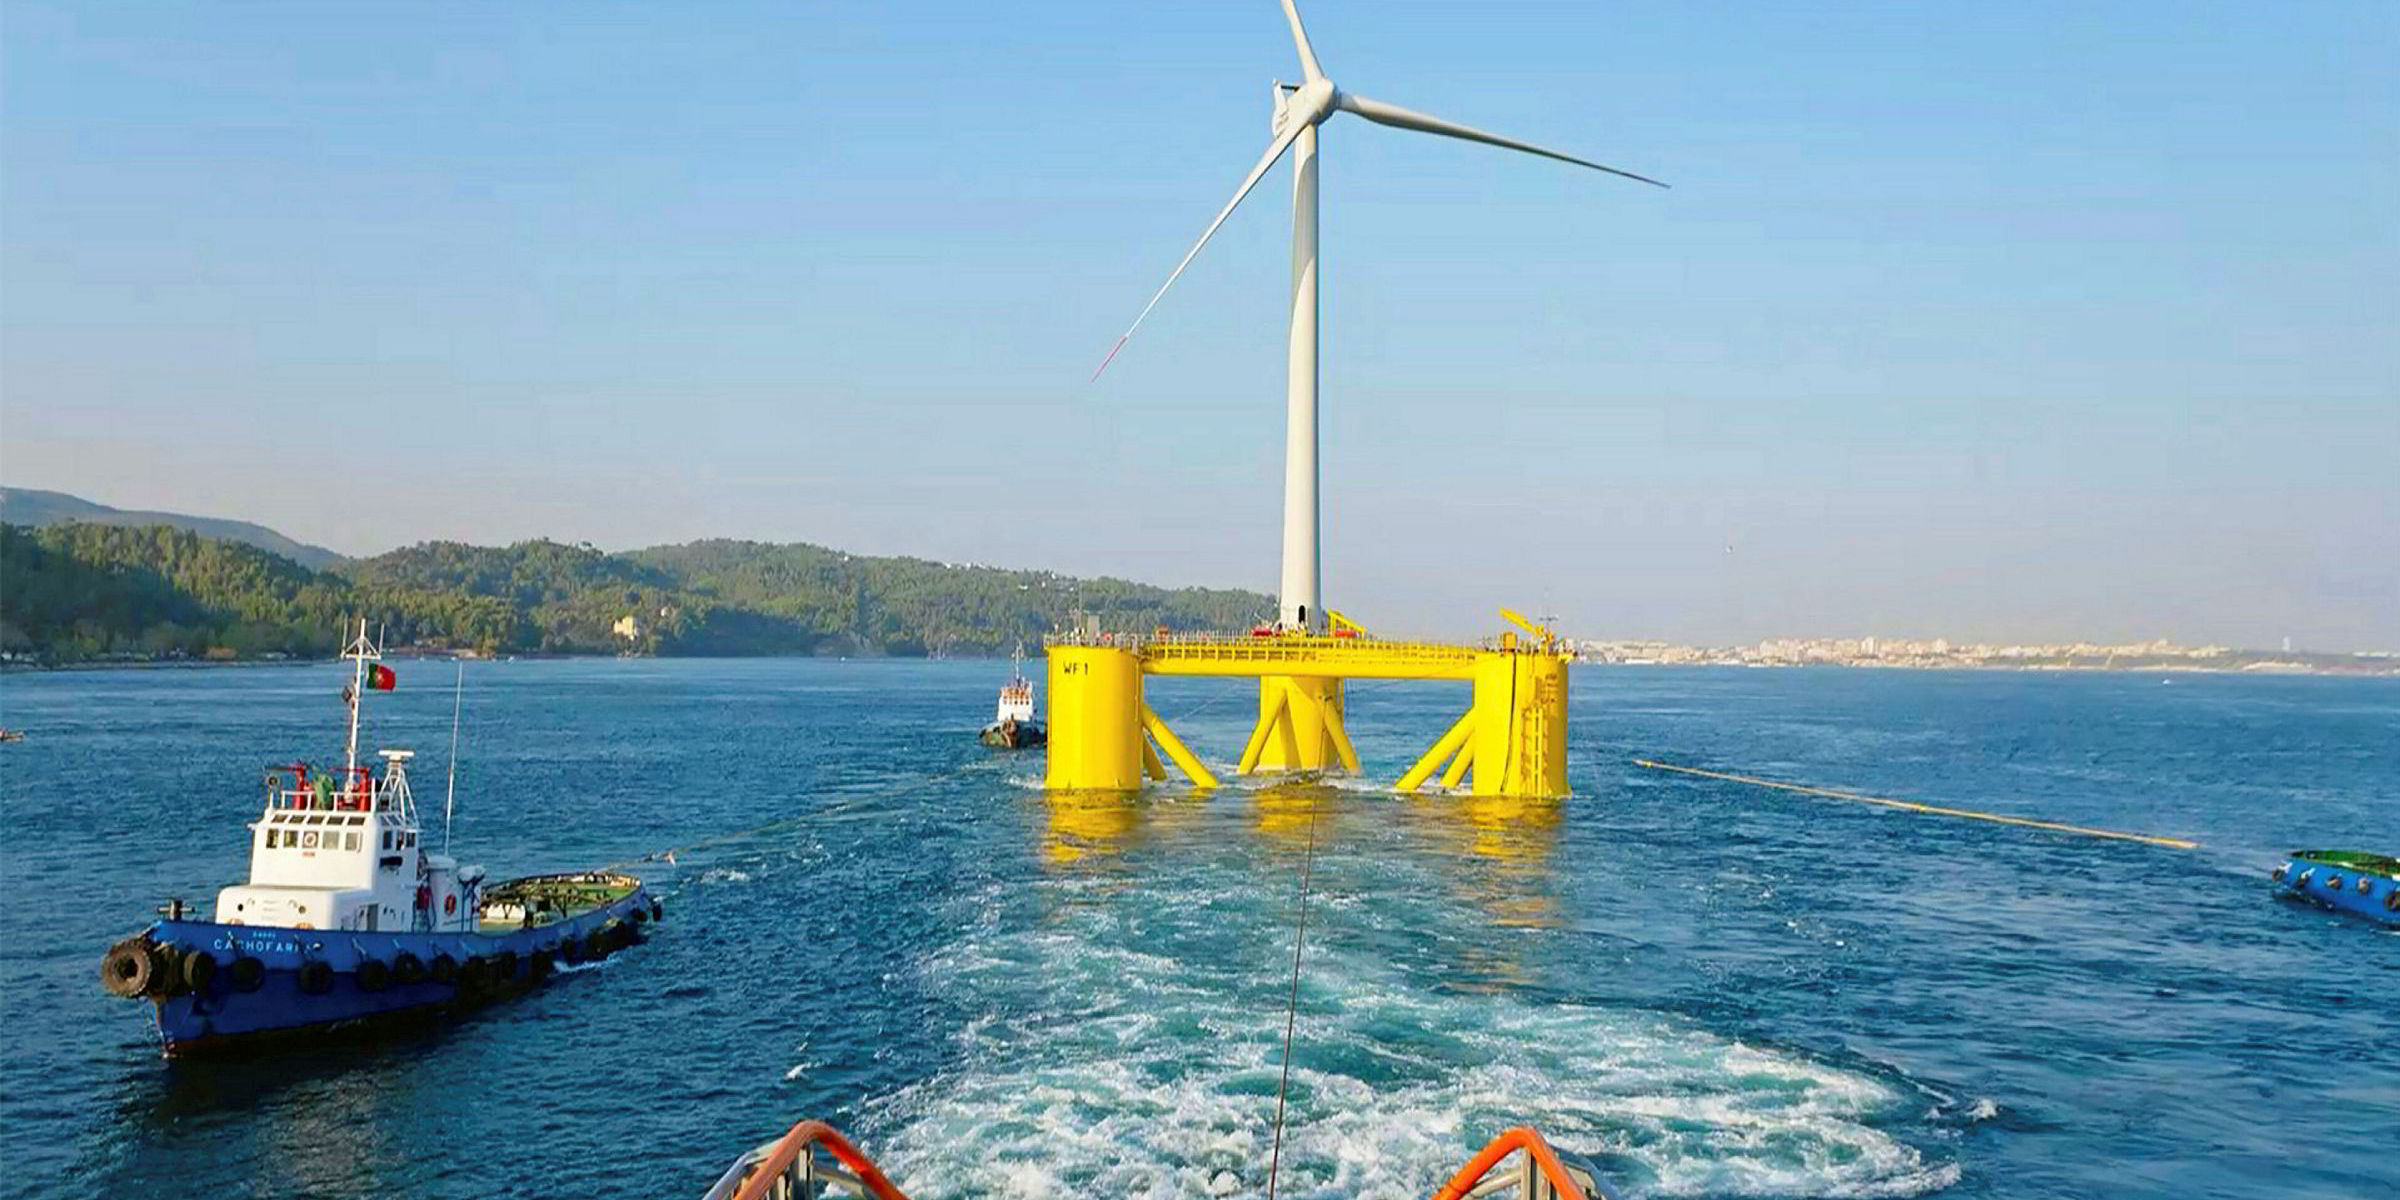
\includegraphics[scale=0.15]{img/WindFloatProject.jpeg}
    \caption{Plateforme situé au Portugal}
    \label{fig:CameraCmdsettings}
\end{figure}

\subsubsection{Contexte}
\subsubsubsection{Le projet WindFloat Atlantic}

Tachyssema Developpement participe au projet WindFloat Atlantique mené par EDP Renewables, Engie, Repsol et Principle Power Inc. Ce projet consite à la réalisation de plateformes exploitants l'énergie éolien offshore. 

\subsubsubsection{Traitement des données utile pour l'asservissement d'une plateforme}
Informations utiles: Le Xsens MTi-10-series est un module qui regroupe un ensemble de capteurs permettant d'obtenir des informations d'une grande précision sur l'orientation, l'inclinaison, les accélérations sur 3 axes ( x,y,z) ainsi que les positions GPS. 
\newline

Les plateformes sont équipés d'un asservissement qui leurs permet de rester stables malgrès des conditions métérologiques pouvant être difficiles comme dans le cas d'une forte houle ou de vents trop importants. Les plateformes sont équipés de trois flotteurs qui assurent leurs bon équilibre. Des pompes à eau sont présentes dans chaque flotteur. L'asservissement agit sur la commande de ces pompes à eau pour maintenir les plateformes en équilibres. 
La positions GPS doivent aussi être connu en temps réel pour vérifier que les plateformes ne dérives pas. 
Toutes ces données proviennent de modules Xsens installées directement sur les plateformes qui transmettent les informations par communication série à un automate qui est lui même relié au sol par via le protocole de communication MODBUS.  (voir figure ci-dessous)
\newpage


\begin{figure}[ht]
    \centering
    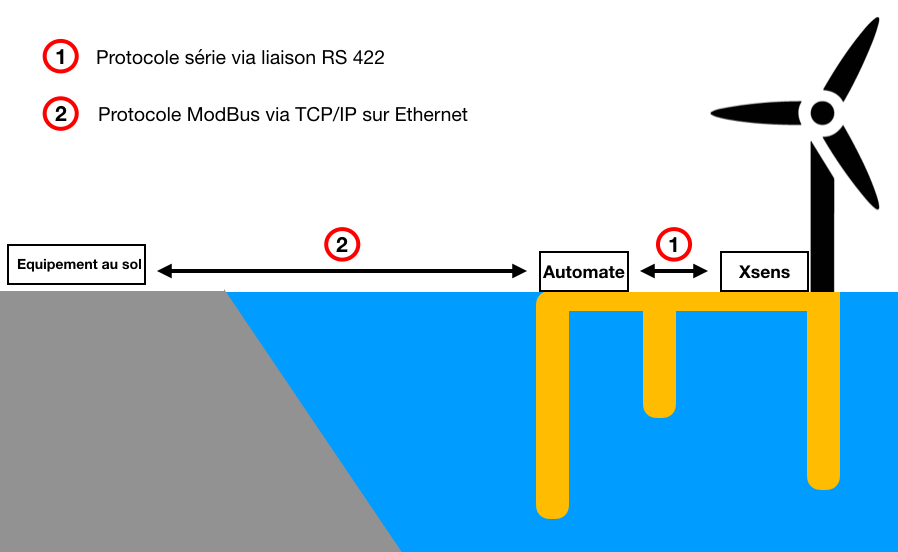
\includegraphics[scale=0.45]{img/schKOWL.png}
    \caption{Illustration de la communication entre équipements }
    \label{fig:CameraCmdsettings}
\end{figure}

\subsubsection{Travail effectué}

Ma mission sur ce projet consistait à : 
\newline
\begin{itemize}
	\item Configurer le module Xsens pour que les données répondants au cahier des charges soient transmises à la bonne fréquence ( qui était initialement de 50 Hz). Les données utiles étaient donc le lacet (yaw), le roulis (roll), le tangage (pitch), la lattitude, la langitude ainsi que les accélérations X,Y et Z. 
	\item Etudier la trame généré par le module Xsens, le fonctionnement de la réception série de l'automate et a transmission des données en provenance de l'automate via le protocole MODBUS. 
	\item Créer un executable en C\# (s'exécutant sur un équipement au sol) permettant de lire les données disponibles sur l'automate et de les interpréter pour reconstituer la trame du module Xsens et enfin d'extraire les informations souhaitées. 

\end{itemize}

\subsection{Etude du protocole MAVLINK }

\subsubsection{Contexte}

Le protocole MAVLINK est un ...

